\documentclass[10pt, letterpaper, notitlepage]{report}
\usepackage{kactlpkg}
\usepackage{mathtools}
\kactlcontentdir{../content}

\university{UFRJ}{Federal University of Rio de Janeiro}{projeto}
\team{UFRJ - Time Feliz \textasciicircum--\textasciicircum}{Chris Ciafrino, Gustavo Miguel e Letícia Freire} 
\contest{adapted from KTH ACM Contest Template Library}{2019}

\begin{document}
	\maketeampage
	% Small KACTL header on the first page:
	%\maketitle{``One Last Time'' Edition}{\today}
	\begin{multicols*}{3}
	\setcounter{tocdepth}{0} % maybe want sections?
	\tableofcontents
	\thispagestyle{fancy}
	\kactlchapter{contest}
	\kactlchapter{math}
	\kactlchapter{misc}
	\kactlchapter{data-structures} \newpage
	\kactlchapter{numerical}\newpage
	\kactlchapter{number-theory}\newpage
	\kactlchapter{combinatorial}\newpage
	\kactlchapter{graph}\newpage
	\kactlchapter{geometry}\newpage
	\kactlchapter{strings}\newpage
	\kactlchapter{various}
	\end{multicols*}

	%\begin{multicols*}{3}
	%\kactlchapter{appendix}
	%\end{multicols*}
\end{document}
\centerline{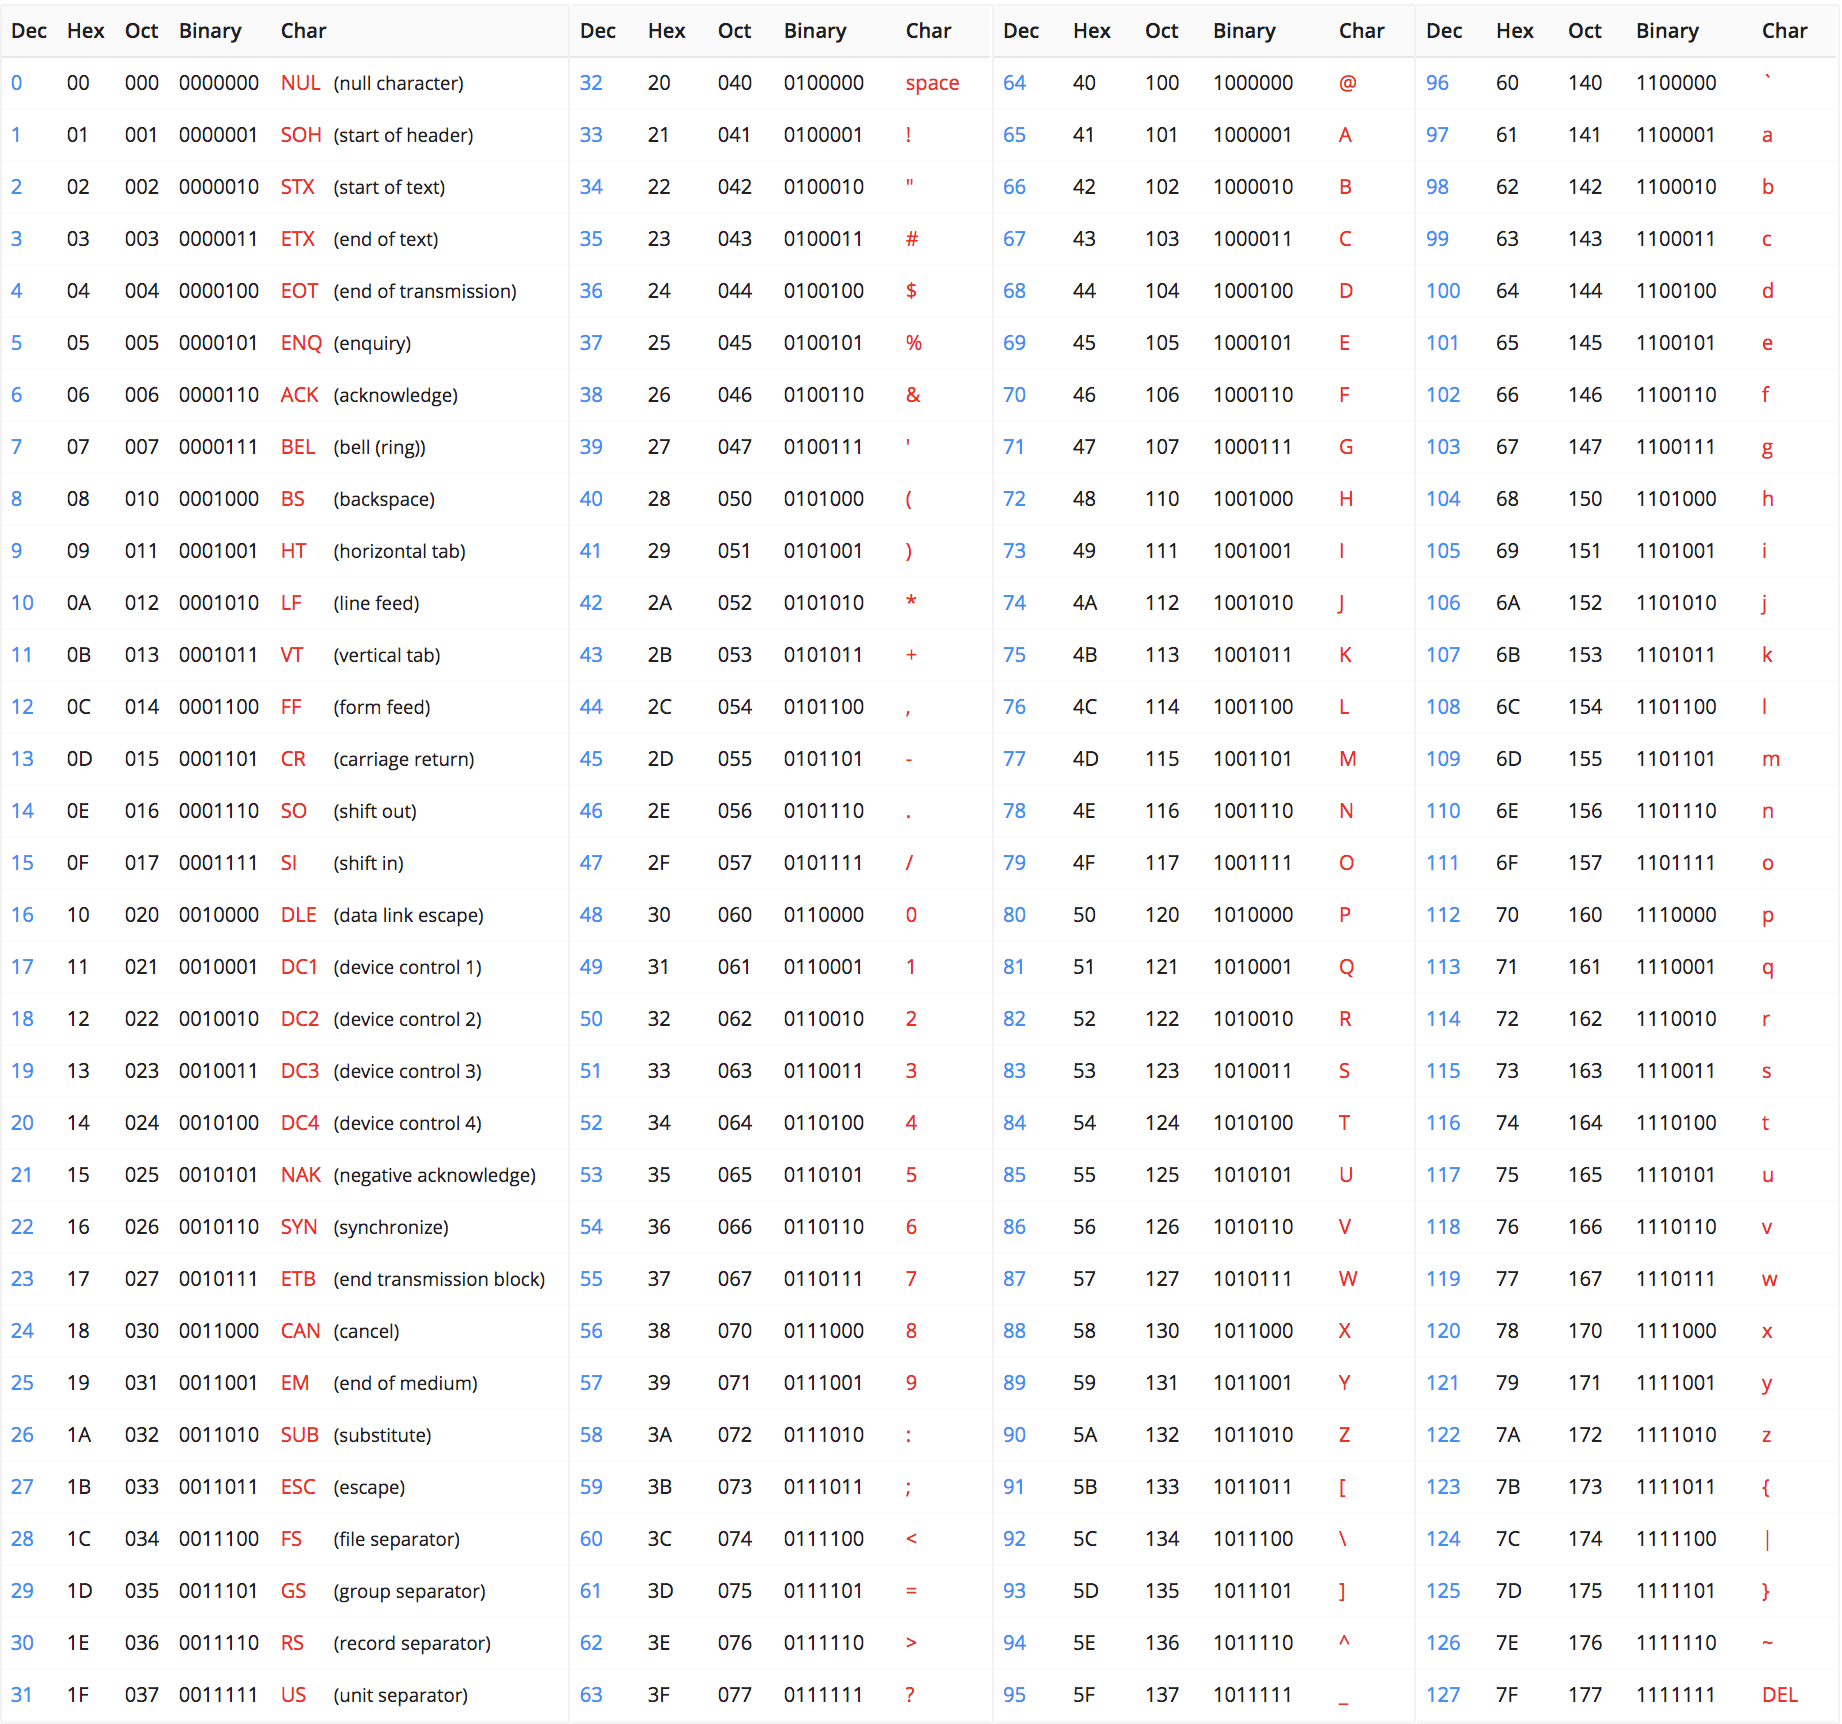
\includegraphics[width=250mm]{../content/various/asciitable}}
